 
   %judul bisa diketik ulang
  \setstretch{1}%\small
  \begin{center}
      \textbf{\large \Title}\\
      \bigskip 
  \end{center}
  
  
  
  %Nama authors
   \begin{center}
     \bf \Author$^1$, Parman Sukarno$^2$, Erwid M. Jadied$^3$ 
  \end{center}
  
  
  %Afiliasi dan email
   \begin{center}
     $^{1,2,3}$Fakultas Informatika, Universitas Telkom, Bandung\\
%$^4$Divisi Digital Service PT Telekomunikasi Indonesia\\
$^1$hasobiroid@student.telkomuniversity.ac.id, $^2$psukarno@telkomuniversity.ac.id,\\ $^3$jadied@telkomuniversity.ac.id %$^4$pembimbingluar@telkom.co.id 
  \end{center}
  
   
 %%% Abstrak Indonesia %%%%%%%%%%  
   
{\bf \parindent0pt \noindent\rule{\textwidth}{1pt}
Abstrak

Perkembangan internet membawa dampak besar bagi kehidupan manusia, tetapi tidak semua hal yang berawal dari internet adalah hal positif. Salah satunya adalah ancaman kejahatan yang bertambah melalui internet atau cybercrime. Salah satu bentuk cybercrime adalah DDoS, DdoS adalah serangan pada jaringan yang sederhana namun efektif, beberapa kerugian besar telah diakibatkan oleh DdoS. Daegan adanya permasalahan diatas maka kebutuhan akan pendeteksian DDoS semakin penting, pada proposal ini diusulkan system pendeteksian DDoS secara Real Time dengan arsitektur Centralized Intrusion Detection System (CIDS) dimana mampu mendeteksi DDoS dengan keakurasian deteksi diatas 80\% \cite{ddosfuzzy}\cite{ddosfpga}\cite{ddosrbf} dan dalam rentan waktu 0 hingga 10 detik.

 \bigskip
Kata kunci : DDoS, Real Time, CIDS



%%% Abstrak English %%%%%%%%%%  



\noindent\rule{\textwidth}{1pt}
Abstract

The abstract should state briefly the general aspects of the subject and the main concolusions.  The length of abstract should bo no more than 200 word and  should be typed be with 10 pts.

 \bigskip
Keywords: keyword should be chosen that they best describe the contents of the paper and should be typed in lower-case, except abbreviation. Keyword should be no more than 6 word 

\noindent\rule{\textwidth}{1pt} }
   


%%%%%% isi paper %%%%

\section{Pendahuluan}

\noindent\textbf{Latar Belakang}

Perkembangan internet dapat dikatakan pesat semenjak pertama kali digunakan untuk kepentingan militer dan akademik di Amerika Serikat, kini internet sudah mencakup segala aspek kehidupan manusia, mulai dari bidang komunikasi, Pendidikan, hiburan, hingga perbankan. Kompleksitas teknologi yang ada didalamnya pun semakin berkembang dari masa ke masa. Selain itu, ancaman kejahatan siber juga sudah muncul dari tahun 1820 meski saat itu belum ada internet. Kejahatan siber modern ini menyasar kepada data-data pribadi seperti alamat email, data kartu kredit, alamat rumah, detil identitas d.l.l.

Salah satu jenis serangan internet adalah DDoS, serangan DDoS pertama kali yang terdokumentasikan adalah pada 7 Februari 2000 yang menimpa beberapa situ e-commerce di Amerika Serikat seperti Amazon, e-Bay. Sejak saat itu serangan DDoS terus berkembang dan berevolusi menjadi lebih efektif  dan berbahaya. Contoh serangan DDoS lain yang menarik perhatian dunia adalah serangan DDoS di Estonia pada tahun 2007, dimana serangan DDoS di negara itu dapat melumpuhkan jaringan internet seluruh negara \cite{politicsofddos}.

Dari kejadian-kejadian diatas, dapat dilihat bahwa DDoS memiliki peran dan tingkat berbahaya yang tinggi, hal ini mendorong peneliti-peneliti di dunia untuk mempelajari DDoS dan melakukan deteksi lebih awal terhadap serangan DDoS. Deteksi serangan dengan DDoS dapat diklasifikasikan menjadi dua kategori, misuse detection dan anomaly detection [3]. Deteksi DDoS yang efektif serta dapat memberikan jaminan kemanan adalah system deteksi yang dapat berjalan secara real time [4]. Dengan diterapkannya sistem real time DDoS detection maka kemungkinan serangan yang dapat menyebabkan kerusakan yang lebih jauh dapat dihilangkan. Selain itu Sistem deteksi DDoS komersial memiliki tingkat alarm palsu yang tinggi, menghasilkan ratusan alarm palsu per hari karena seringkali sulit untuk memilih secara manual kondisi identifikasi untuk sejumlah besar serangan dan varian mereka[9].

Shiaeles, Katos, Karakos a, Papadopoulos[4] mengembangkan Real Time DDoS Detection dengan menggunakan fuzzy estimator dan dapat menghasilkan akurasi 80\%. Sedangkan Hoque, Kashyap, Bhattacharyya[6] melakukan Real Time DDoS Detection dengan metode FPGA (Field Programmable Gate Arrays) mampu mendeteksi dengan tingkat akurasi mencapai 100\% dengan menggunakan NaHiDVERC (NaHiD for DDoS detection using Variation, Entropy of Source IPs and Packet Rate) yang diterapkan menggunakan FPGA, namun DDoS oleh NaHiDVERC masih dianggap sebagai masalah kelas dua, sehingga masih harus ada perbaikan. Namun, ketiga metode diatas masih dapat dikembangkan untuk mencapai akurasi deteksi yang lebih baik lagi dengan metode yang berbeda digabungkan dengan arsitektur IDS yang tepat.

Centralized Intrusion Detection System (CIDS) adalah suatu system pendeteksian serangan yang terpusat, menjadikannya mudah untuk memonitor serta melihat hasil laporan dan data serangan yang terjadi pada suatu jaringan. Dengan teknik pendekteksian DDoS, yakni teknik Real Time dan IDS yang tercentralisasi (CIDS) diharapkan dapat meningkatkan akurasi pendeteksian dan kecepatan deteksi.\\


\noindent\textbf{Topik dan Batasannya}

\begin{enumerate}
    \item Menggunakan arsitektur Centralized Intrusion Detection System (CIDS).
    \item Range waktu deteksi ditentukan dari awal.
    \item Menggunakan algoritma \textit{Artificial Neural-Network}
\end{enumerate}

\noindent\textbf{Tujuan}

\begin{itemize}
    
    \item Mengukur akurasi deteksi DDoS menggunakan CIDS dan Neural-Network
    \item Membuat data yang tidak terstruktur menjadi terstruktur.
    \item Mengukur waktu deteksi

\end{itemize}
\begin{comment}
\noindent \textbf{Organisasi Tulisan}

Pada sub-bagian ini dituliskan bagian-bagian selanjutnya (setelah Pendahuluan) pada jurnal TA ini, disertai penjelasan sangat singkat.
\end{comment}

\section{Studi Terkait}

\subsection{Real Time DDoS Detection}

Real Time DDoS Detection adalah metode dalam pendeteksian DDoS dengan acuan waktu tertentu, waktu yang ditetapkan memiliki Batasan yang jelas \cite{ddosfuzzy} sehingga hasil yang dihasilkan memenuhi kriteria-kriteria yang telah ditetapkan sebelumnya.
Pendeteksian DDoS yang tidak berdasarkan Real Time cenderung memiliki tingkat deteksi yang lebih lambat\cite{ddosfuzzy}.

Pustaka \cite{ddosfpga} menyatakan bahwa Real Time DDoS harus mengidentifikasi serangan dengan overhead komputasi yang rendah. Meskipun sejumlah besar metode statistik telah dirancang untuk deteksi serangan DDoS, solusi real time untuk mendeteksi serangan DDoS di perangkat keras masih bias dikatakan sedikit.

Pustaka \cite{ddosfuzzy}\cite{ddosfpga} melakukan percobaan Real Time DDoS Detection menggunakan dua algoritma yang berbeda yakni Fuzzy Estimators dan FPGA tetapi tidak melakukan perubahan atau modifikasi pada aristektur IDS. Sedangkan modifikasi yang dapat dilakukan pada bagian IDS selain algoritma adalah aristektur.

Real Time DDoS Detection menjanjikan hasil yang akurat dalam rentang waktu tertentu\cite{ddosfuzzy}. Real Time DDoS Detection akan mendeteksi serangan DDoS dengan metode TCP,UDP, dan ICMP flooding karena ketiga metode tersebut adalah metode yang terefektif menyebabkan sumber daya tidak dapat diakses\cite{ddosstat}.



\subsection{Arsitektur}
\subsubsection{Distributed Intrusion Detection System}

Distributed Intrusion Detection System (DIDS) terdiri dari beberapa IDS yang terdapat pada jaringan besar, yang kesemuanya berkomunikasi satu sama lain, atau dengan server pusat yang memfasilitasi pemantauan jaringan tingkat lanjut\cite{dids1}. DIDS memiliki keuntungan salah satunya adalah kinerja hardware yang cenderung lebih ringan disbanding CIDS karena beban kerja dibagi berdasarkan prinsip terdistribusi.

Pada DIDS cenderung sukar untuk menerapkan metode Real Time detection karena analisis serta lokasi-lokasi untuk menganalisis data yang diperoleh dilakukan pada beberapa lokasi sesuai dengan prinsip terdistribusi \cite{idssurvey}.


\subsubsection{Centralized Intrusion Detection System}

Centralized Intrusion Detection System (CIDS) menawarkan hasil yang bagus dengan estimasi deteksi antara tiga gingga tujuh detik\cite{cids1}. Selain itu pengaturan dan monitorin dari system juga dapat dijalankan lebih mudah karena analisis dari data serangan yang diperoleh telah ditetapkan pada lokasi-lokasi tertentu \cite{idssurvey}.  CIDS juga mampu melindungi jaringan dari berbagai serangan internet selain DoS, seperti Probe dan worm ketika serangan internet telah terdeteksi.

CIDS juga dapat menjadi stand-alone IDS atau collaborative software dengan beberapa software pendeteksi lain[10]. Dibalik kemudahan yang ditawarkan oleh CIDS ada beberapa masalah yang timbul seperti, cost yang lebih tinggi, kinerja hardware yang lebih berat dari DIDS serta resource yang dibutuhkan lebih besar dibandingkan dengan DIDS.





\subsection{Algoritma}
\subsubsection{Artifical Neural Network}
    Beberapa algoritma yang telah digunakan untuk mendeteksi DDoS diantaranya \textit{Fuzzy Estimators}, FPGA (\textit{Field Programmable Gate Arrays}), namun pada karya ilmiah kali ini algoritma yang akan digunakan adalah \textit{Artificial Neural Network} (ANN).
    
    Penggunaan ANN memiliki beberapa keunggulan yakni, XXXX sehingga apabila diterapkan pada \textit{Centralized Intrusion Detection System} (CIDS) diharapakan akan menghasilkan XXX

\subsection{Network Time Protocol}

Sinkronisasi waktu jaringan mengacu pada penyimpangan batas waktu yang dilakukan oleh berbagai komunikasi atau komputer perangkat dalam jaringan dalam rentang yang cukup kecil\cite{ntp1}, sinkronisasi waktu pada jaringan dan server dapat dilakukan dengan berbagai metode, salah satunya adalah NTP. Keunggulan dari NTP memiliki akurasi tinggi serta dapat menggunakan berbagai alat sebagai referensi waktu seperti GPS, Time Code d.l.l. NTP bekerja dengan cara klien NTP memulai pertukaran permintaan waktu dengan server NTP. Sebagai hasil dari pertukaran ini, klien dapat menghitung penundaan tautan dan offset lokalnya, dan menyesuaikan jam lokal agar sesuai dengan jam di komputer server.

Dibandingkan dengan protokol lainnya untuk sinkronisasi waktu seperti SNTP (Simple Network Time Protocol), NTP dapat lebih andal karena dapat menerima input waktu dari berbagai sumber sedangkan SNTP hanya dapat menggunakan satu sumber input waktu, dari jam hardware atau jam interface jaringan. Namun, kedua protocol ini dapat bertukar informasi mengenai waktu sehingga lebih memudahkan dalam perancangan sistem.


\subsection{Distributed Denial of Service}

%\subsection{Botnet (?)}

\subsection{Dataset}

Dataset yang akan digunakan adalah NSL KDD \texttt{(github.com/defcom17/NSL\_KDD)} karena dataset KDD lama sudah tidak diperbaharui lagi sejak 1999 sehingga sudah tidak relevan dengan gambaran serangn DDoS saat ini.

\subsection{Server}
\subsubsection{Operating System}

\textit{Operating System} yang akan digunakan adalah Linux OS dengan Ubuntu versi 18.04

\subsubsection{Web Server}
Apache2
\subsubsection{Database Server}
Mysql

\subsubsection{IDS (\textit{Intrusion Detection System})}
Snort

\begin{comment}
\subsubsection{Arsitektur Hadoop dan HBase}

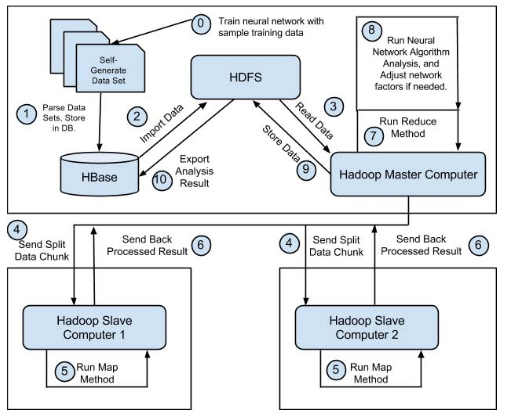
\includegraphics[scale=0.7]{hadoop-architecture.png}
\end{comment}
\subsection{Topologi}

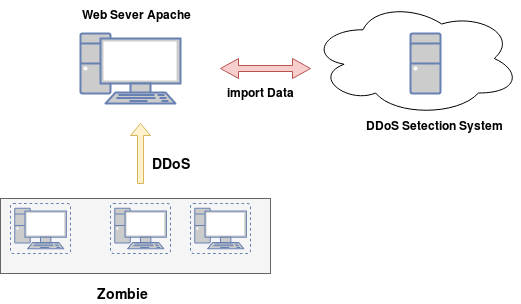
\includegraphics[scale=0.7]{diagram-web.png}

\section{Pengujian}



\section{Evaluasi}

   
\section{Kesimpulan}
 
 


\bibliographystyle{abbrv}
\bibliography{references}

\section*{Lampiran}

\noindent Lampiran dapat berupa detil data dan contoh lebih lengkapnya, data-data pendukung, detail hasil pengujian, analisis hasil pengujian, detail hasil survey, surat pernyataan dari tempat studi kasus, screenshot tampilan sistem, hasil kuesioner dan lain-lain.